% Written with Elsevier's elsarticle LaTeX template (elsarticle.cls),
% the template for the Journal of Financial Economics and other Elsevier journals.
\documentclass[preprint,letterpaper,11pt,authoryear]{elsarticle}
\usepackage{lmodern}
\usepackage[margin=1in]{geometry}
\usepackage{amsmath}
\usepackage{graphicx}
\usepackage{booktabs}
\usepackage{array}
\usepackage[hidelinks]{hyperref}
\hypersetup{pdftitle={Entrepreneur Debt Aversion and Bank Borrowing: A Replication of Paaso, Pursiainen and Torstila (2025)},pdfauthor={Nowshed Hossain Imran}}

% Notes printed under a table or figure
\newenvironment{tablenotes}{\par\vspace{3pt}\begin{minipage}{0.95\linewidth}\footnotesize\textit{Note:} }{\end{minipage}}
\newenvironment{figurenotes}{\par\vspace{3pt}\begin{minipage}{0.95\linewidth}\footnotesize\textit{Note:} }{\end{minipage}}

% Footer on the first page
\myfooter[L]{Replication paper, ECON 5213 Econometric Analysis, Oklahoma State University, in progress, October 2026}

\begin{document}
\setlength{\emergencystretch}{2em}

% let tables share a page with text instead of sitting alone on a float page
\renewcommand{\topfraction}{0.9}
\renewcommand{\textfraction}{0.1}
\renewcommand{\floatpagefraction}{0.8}

\begin{frontmatter}

\title{Entrepreneur Debt Aversion and Bank Borrowing: A Replication of Paaso, Pursiainen and Torstila (2025)}

\author{Nowshed Hossain Imran}
\affiliation{organization={Spears School of Business, Oklahoma State University},
             city={Stillwater},
             state={OK},
             country={USA}}

\begin{abstract}
Paaso, Pursiainen and Torstila (2025) survey 917 Finnish owner-managers in 2020 and find that entrepreneurs who dislike debt run firms that use less of it, and were less likely to apply for a bank loan during COVID-19. I replicate their Tables 1, 3A, 4 and 10A with the authors' survey data and my own Stata code. High debt aversion lowers the probability of having debt by 0.093 (clustered standard error 0.027), against 0.094 (0.030) in the paper, and every coefficient in Tables 3A, 4 and 10A is within 0.001 of the paper's. The extension tests the assumptions behind these linear probability models; this version reports five of the six tests, and the instrumental variables test for measurement error is added in the final version. The debt use result survives probit and logit (average partial effect $-0.094$), weighted least squares ($-0.062$), score dummies and the 2023 survey ($-0.196$). However, the bank loan result is weaker: it is $-0.046$ with $p = 0.053$ in the paper's model, and it is not significant in the logit. The score works more like a threshold at 7 and above than a straight line. Debt aversion is a reliable predictor of debt use, and a less reliable one of loan applications.
\end{abstract}

\begin{keyword}
Debt aversion \sep Small business finance \sep Linear probability model \sep Replication
\JEL G32 \sep D91
\end{keyword}

\end{frontmatter}

\section{Introduction}

When COVID-19 closed much of Europe in spring 2020, governments offered small firms loans backed by state guarantees. Many firms that needed cash did not take them. Paaso, Pursiainen and Torstila (2025) ask whether part of the reason sits in the owner's head. Corporate finance theory treats debt as a neutral tool, but many people see borrowing as something shameful or dangerous, and the owner of a small firm is the one who decides whether the firm borrows. If owners who dislike debt avoid it even when the firm needs money, then policies built on loans will reach fewer firms than planned.

I ask two questions. The first is whether I can reproduce the paper's main estimates with my own code. The second is whether the estimates hold when the assumptions of the linear probability model are tested. I follow the cross-section workflow in Wooldridge (2020): I estimate the paper's models by ordinary least squares with clustered standard errors, compare them with probit and logit, test for heteroskedasticity and estimate weighted least squares, test the functional form of the debt aversion score, and test whether the effect differs across groups of owners. The instrumental variables test for measurement error in the score is added in the final version, after chapter 15 is covered in class.

The replication works. Every coefficient in Tables 3A, 4 and 10A of the paper is reproduced to within 0.001. The debt use result also holds in every test of the extension reported here. However, the bank loan result is weaker than the paper suggests, it depends on the estimator and is significant at the 5 percent level only under weighted least squares.

\section{Original Study and Mechanism}

The paper studies 917 Finnish firms whose survey respondent is also the owner. The key variable is the owner's answer, on a scale from 0 (disagree completely) to 10 (agree completely), to the statement ``I consider taking on debt to be unpleasant.'' Owners who answer 8, 9 or 10 are coded as having high debt aversion, which is about 45 percent of the sample. The outcomes are whether the firm has debt now, whether it had debt in the past five years, and whether it applied for a new bank loan during the COVID-19 crisis.

The mechanism is a preference, not a constraint. A debt-averse owner gets a personal cost from borrowing that a profit-maximizing firm would not have, so the owner borrows less at any interest rate. The COVID-19 shock helps the argument. The Finnish support for small firms ran mainly through bank loans with a government guarantee of 50 to 80 percent, and the shock came suddenly to most firms at the same time. Thus a debt-averse owner could not have chosen in advance a firm with low financing needs.

The main threat is that debt aversion is not randomly assigned. An owner who had a bad experience with debt, or whose firm is riskier, may both dislike debt and borrow less for reasons the survey does not record. The paper answers this with controls for risk appetite, optimism and trust, with fixed effects for firm and owner characteristics, and with a survey experiment that labels the same support policy as a loan or as a grant. I replicate the regression part and leave the experiment aside. The paper reports that high debt aversion lowers the probability of having debt by about 9 percentage points against a base rate of 48 percent.

\section{Data}

The data are the authors' own survey, run by TNS Kantar between 27 May and 8 June 2020 among members of the Federation of Finnish Enterprises and firms in the Bisnode Finland database. Of the 1,008 firms that answered, the authors keep the 917 whose respondent is an owner-manager. The cleaned survey file comes from the paper's replication package at the journal (Paaso et al. 2025), and the authors agreed to its use for this extension. The license does not allow the data to be shared, so the data files are not in the project repository. The package also contains a 2023 follow-up survey of 1,041 firms, which the paper uses in Table 10.

The unit of observation is a firm, and the sample is one cross-section. Most firms are small: 38.6 percent have one employee and 2.6 percent have more than 50. Table~\ref{tab:summary} shows the main variables. My means and standard deviations are the same as the paper's Table 1 to the third decimal for every variable I checked, which means the cleaned file is the one the authors used. The paper's Table 3B uses debt ratios from the Orbis database, and those variables were removed from the package for license reasons, so Table 3B cannot be replicated.

\begin{table}[!htbp]
\centering\small\setlength{\tabcolsep}{5pt}
\caption{Summary Statistics, 2020 Survey}
\label{tab:summary}
\begin{tabular}{lcccc}
\toprule
Variable & Mean & SD & Median & $N$ \\
\midrule
Has debt (0/1) & 0.480 & 0.500 & 0 & 917 \\
Had debt in the past 5 years (0/1) & 0.606 & 0.489 & 1 & 917 \\
Applied for a new bank loan during COVID-19 (0/1) & 0.156 & 0.363 & 0 & 917 \\
High debt aversion (0/1) & 0.449 & 0.498 & 0 & 899 \\
Debt aversion (0 to 10) & 6.337 & 2.894 & 7 & 899 \\
Risk appetite (0 to 10) & 5.976 & 2.169 & 6 & 904 \\
Optimism (0 to 10) & 7.255 & 1.923 & 8 & 901 \\
Distrust people (0 to 10) & 5.406 & 2.653 & 6 & 903 \\
Distrust banks (0 to 10) & 5.132 & 2.769 & 5 & 907 \\
\bottomrule
\end{tabular}
\begin{tablenotes}
Owner-managers only. Every value matches the paper's Table 1. Eighteen owners did not answer the debt aversion question. Source: \texttt{output/table1\_summary\_stats.csv}.
\end{tablenotes}
\end{table}

Figure~\ref{fig:score} shows the share of firms with debt at each value of the score. For most scores up to 6, more than half of the firms have debt, and for every score from 7 to 10 the share is below half. The exception is a score of 3, but only 71 owners chose it. The picture already suggests, the relationship is closer to a step than to a straight line, which Section~\ref{sec:ext} tests.

\begin{figure}[!htbp]
\centering
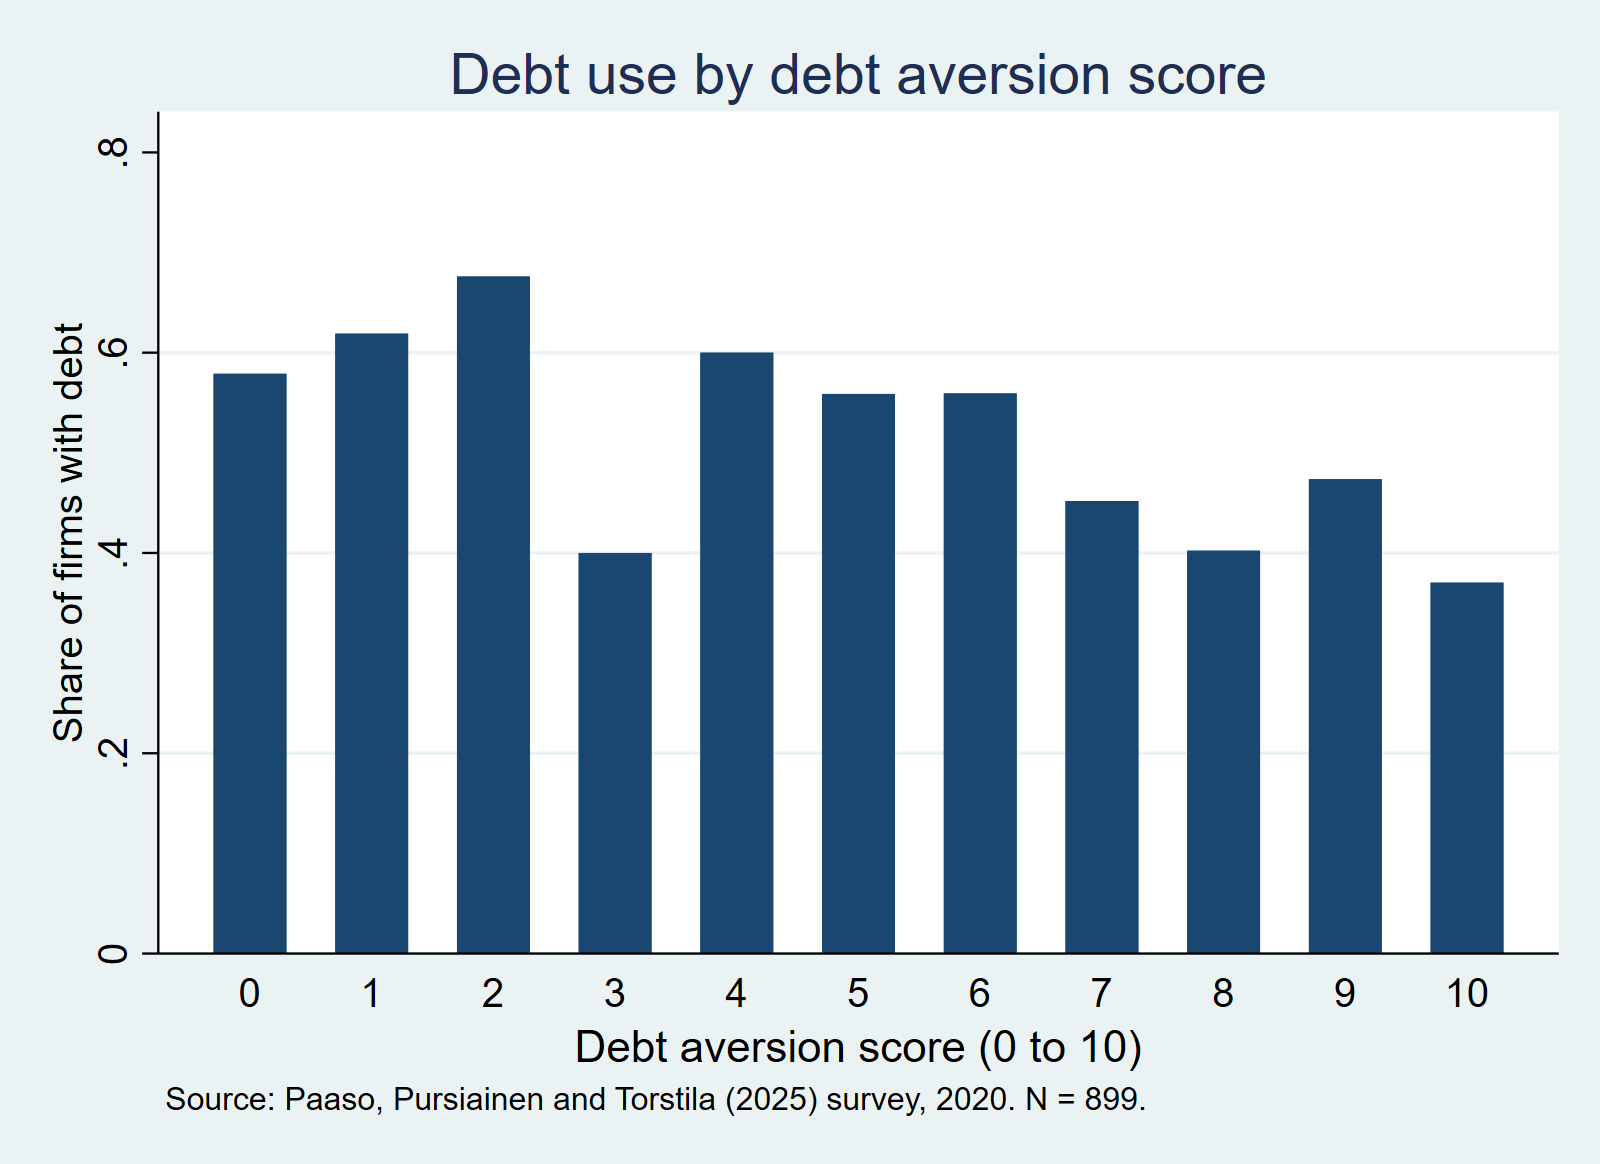
\includegraphics[width=0.62\linewidth]{fig1_debt_by_score.png}
\caption{Share of Firms with Debt by Debt Aversion Score}
\label{fig:score}
\begin{figurenotes}
Raw shares, no controls, $N = 899$. The cells at the low end are small: 38, 21, 71, 55 and 45 owners chose scores 0 to 4. Source: \texttt{output/fig1\_debt\_by\_score.png}.
\end{figurenotes}
\end{figure}

\section{Empirical Strategy}

The paper's model is a linear probability model,
\begin{equation}
\label{eq:lpm}
y_i = \beta_0 + \beta_1 \, HDA_i + \gamma_1 \, risk_i + \gamma_2 \, opt_i + \gamma_3 \, dpeople_i + \gamma_4 \, dbanks_i + \mathbf{d}_i\boldsymbol{\delta} + u_i,
\end{equation}
where $y_i$ is a 0/1 outcome for firm $i$, $HDA_i$ is the high debt aversion indicator, the four traits are risk appetite, optimism, distrust of people and distrust of banks, and $\mathbf{d}_i$ is a set of dummies for firm size, industry, the owner's expectation of firm survival and survival time, and the owner's field and level of education. In other columns $HDA_i$ is replaced by the 0 to 10 score. The paper absorbs the dummies with a fixed effects command; I include them directly with \texttt{reg y x i.var}, which gives the same coefficients. Firms that are alone in a category are dropped, as the paper does. The standard errors are clustered by the firm's municipality (44 clusters), which allows the errors of firms in the same place to be correlated.

The identifying assumption is $E(u_i \mid HDA_i, \mathbf{x}_i) = 0$: after the traits and the dummies, debt aversion is not related to anything else that affects borrowing. The replication tests three hypotheses from the paper.
\begin{itemize}
\item H1. Owners with high debt aversion are less likely to have debt now and to have had debt in the past five years (paper's Table 3A).
\item H2. Owners with high debt aversion were less likely to apply for a new bank loan during COVID-19 (Table 4).
\item H3. The effect on debt use holds in the 2023 survey (Table 10A).
\end{itemize}

The extension asks whether the estimates depend on the assumptions of the linear probability model. I test six hypotheses on the main specifications, which are column (2) of Table 3A for having debt and column (2) of Table 4 for the bank loan.
\begin{itemize}
\item H4. The effect of high debt aversion is the same in a probit or logit model as in the linear model.
\item H5. The errors of the linear model are homoskedastic, and weighted least squares gives the same effect.
\item H6. The effect of the 0 to 10 score is linear.
\item H7. The score is measured without error, so ordinary least squares is not biased toward zero (instrumental variables; added in the final version).
\item H8. The effect of high debt aversion is the same for women and men, and for firms with fewer than 5 employees and larger firms.
\item H9. In the 2023 survey, the effect is the same in a probit or logit model as in the linear model.
\end{itemize}

For H4 and H9, a linear probability model can give fitted values below 0 or above 1, and it assumes the effect is the same for every firm. Probit and logit avoid both, and I compare their average partial effects with $\beta_1$ (Wooldridge 2020). For H5, the variance of a 0/1 outcome is $p(\mathbf{x})[1 - p(\mathbf{x})]$, so the errors of the linear model must be heteroskedastic. I run the Breusch-Pagan test and the special form of the White test, then estimate weighted least squares with $h_i = \hat{y}_i(1 - \hat{y}_i)$ and keep the clustered standard errors. Fitted values outside 0 and 1 are set to 0.01 and 0.99.

For H6, I replace the score with ten dummies for each value and test the nine restrictions that make the dummies a straight line, $\beta_k = k\,\beta_1$ for $k = 2$ to 10. I also add a squared score and run the RESET test. For H8, I interact high debt aversion with a female indicator and with a larger-firm indicator and test the interaction, and I also run a Chow test that compares the model in each group with the pooled model.

\section{Replication Results}

\subsection{Debt use and bank loans}

Table~\ref{tab:t3} shows the replication of Table 3A. Without controls, owners with high debt aversion are 13.5 percentage points less likely to have debt. With the traits and the dummies, the gap falls to 9.3 points, with a clustered standard error of 0.027. A one point higher score lowers the probability by 1.9 points. The same pattern holds for debt in the past five years. Risk appetite is the only trait with a significant effect on current debt (0.015, significant at 5 percent), and it has the expected sign. H1 is supported.

\begin{table}[!htbp]
\centering\footnotesize\setlength{\tabcolsep}{2.5pt}
\caption{Replication of Table 3, Panel A: Debt Use}
\label{tab:t3}
\begin{tabular}{lcccccccc}
\toprule
 & \multicolumn{4}{c}{Has debt} & \multicolumn{4}{c}{Had debt in the past 5 years} \\
\cmidrule(lr){2-5}\cmidrule(lr){6-9}
 & (1) & (2) & (3) & (4) & (5) & (6) & (7) & (8) \\
\midrule
High debt aversion & $-0.135^{***}$ & $-0.093^{***}$ & & & $-0.128^{***}$ & $-0.089^{***}$ & & \\
 & (0.032) & (0.027) & & & (0.027) & (0.020) & & \\
Debt aversion (0 to 10) & & & $-0.025^{***}$ & $-0.019^{***}$ & & & $-0.024^{***}$ & $-0.020^{***}$ \\
 & & & (0.005) & (0.005) & & & (0.004) & (0.003) \\
Risk appetite & & $0.015^{**}$ & & $0.013^{*}$ & & $0.013^{*}$ & & 0.011 \\
 & & (0.007) & & (0.008) & & (0.008) & & (0.007) \\
Optimism & & 0.007 & & 0.006 & & $-0.002$ & & $-0.002$ \\
 & & (0.008) & & (0.008) & & (0.008) & & (0.008) \\
Distrust people & & $0.009^{*}$ & & $0.009^{*}$ & & 0.007 & & 0.007 \\
 & & (0.005) & & (0.005) & & (0.005) & & (0.005) \\
Distrust banks & & $-0.006$ & & $-0.005$ & & $-0.008$ & & $-0.007$ \\
 & & (0.005) & & (0.005) & & (0.006) & & (0.006) \\
\midrule
Dummies & No & Yes & No & Yes & No & Yes & No & Yes \\
$N$ & 899 & 884 & 899 & 884 & 899 & 884 & 899 & 884 \\
$R^2$ & 0.018 & 0.212 & 0.021 & 0.214 & 0.017 & 0.231 & 0.021 & 0.235 \\
\bottomrule
\end{tabular}
\begin{tablenotes}
Linear probability models. Dummies are firm size, industry, expected firm survival, survival time, and the owner's education field and level. Standard errors clustered by municipality (44 clusters) in parentheses. $^{*}p<0.10$, $^{**}p<0.05$, $^{***}p<0.01$. Source: \texttt{output/table3a\_debt\_use.csv}.
\end{tablenotes}
\end{table}

Table~\ref{tab:t4} shows Table 4. Without controls, owners with high debt aversion were 5.8 points less likely to apply for a new bank loan, against a base rate of 15.6 percent. With the controls the effect is 4.6 points ($p = 0.053$), and it is 4.4 points when the two dummies for the size of the sales shock and the expected time to recover are added. The 0 to 10 score is not significant in any column. Risk appetite raises the probability of applying in every column with controls. Thus H2 is supported only at the 10 percent level, which is also what the paper reports.

\begin{table}[!htbp]
\centering\small\setlength{\tabcolsep}{4pt}
\caption{Replication of Table 4: Applied for a New Bank Loan during COVID-19}
\label{tab:t4}
\begin{tabular}{lcccccc}
\toprule
 & (1) & (2) & (3) & (4) & (5) & (6) \\
\midrule
High debt aversion & $-0.058^{**}$ & $-0.046^{*}$ & $-0.044^{*}$ & & & \\
 & (0.025) & (0.023) & (0.024) & & & \\
Debt aversion (0 to 10) & & & & $-0.007$ & $-0.006$ & $-0.006$ \\
 & & & & (0.005) & (0.004) & (0.004) \\
Risk appetite & & $0.011^{*}$ & $0.011^{*}$ & & $0.011^{*}$ & $0.011^{*}$ \\
 & & (0.006) & (0.006) & & (0.005) & (0.005) \\
\midrule
Dummies & No & Yes & Yes, plus shock & No & Yes & Yes, plus shock \\
$N$ & 899 & 884 & 884 & 899 & 884 & 884 \\
$R^2$ & 0.006 & 0.178 & 0.186 & 0.003 & 0.177 & 0.185 \\
\bottomrule
\end{tabular}
\begin{tablenotes}
Linear probability models. Columns (2), (3), (5) and (6) also control for optimism, distrust of people and distrust of banks, which are not significant. ``Plus shock'' adds dummies for the sales impact of COVID-19 and the expected time to return to normal. Clustered standard errors in parentheses. $^{*}p<0.10$, $^{**}p<0.05$, $^{***}p<0.01$. Source: \texttt{output/table4\_new\_bank\_loan.csv}.
\end{tablenotes}
\end{table}

\subsection{The 2023 survey and benchmark}

In the 2023 survey the paper uses heteroskedasticity-robust standard errors and dummies for industry, firm size and legal form. High debt aversion lowers the probability of having debt by 22.8 points without the dummies and 19.6 points with them, both with a standard error of about 0.03, and the score lowers it by 5.1 and 4.4 points per unit. The effect is about twice as large as in 2020. H3 is supported.

Table~\ref{tab:benchmark} sets my estimates beside the paper's. All 18 coefficients agree to the third decimal or differ by 0.001. My sample in the models with dummies has 884 firms against the paper's 883, and some of my clustered standard errors are smaller in the third decimal, the largest gap is 0.020 against 0.025 in column (6) of Table 3A. I could not find which firm makes the difference. A likely reason is the way the paper's fixed effects command drops singletons and counts degrees of freedom, which my \texttt{reg} code can follow only approximately.

\begin{table}[!htbp]
\centering\small\setlength{\tabcolsep}{4pt}
\caption{Benchmark Comparison with the Paper}
\label{tab:benchmark}
\begin{tabular}{llcc}
\toprule
Table and column & Variable & Paper & Replication \\
\midrule
3A (1) Has debt & High aversion & $-0.135$ (0.033) & $-0.135$ (0.032) \\
3A (2) Has debt & High aversion & $-0.094$ (0.030) & $-0.093$ (0.027) \\
3A (3) Has debt & Score & $-0.025$ (0.005) & $-0.025$ (0.005) \\
3A (4) Has debt & Score & $-0.019$ (0.005) & $-0.019$ (0.005) \\
3A (5) Had debt 5y & High aversion & $-0.128$ (0.031) & $-0.128$ (0.027) \\
3A (6) Had debt 5y & High aversion & $-0.090$ (0.025) & $-0.089$ (0.020) \\
3A (7) Had debt 5y & Score & $-0.024$ (0.004) & $-0.024$ (0.004) \\
3A (8) Had debt 5y & Score & $-0.020$ (0.004) & $-0.020$ (0.003) \\
4 (1) Bank loan & High aversion & $-0.058$ (0.026) & $-0.058$ (0.025) \\
4 (2) Bank loan & High aversion & $-0.047$ (0.025) & $-0.046$ (0.023) \\
4 (3) Bank loan & High aversion & $-0.045$ (0.024) & $-0.044$ (0.024) \\
4 (4) Bank loan & Score & $-0.007$ (0.005) & $-0.007$ (0.005) \\
4 (5) Bank loan & Score & $-0.006$ (0.005) & $-0.006$ (0.004) \\
4 (6) Bank loan & Score & $-0.006$ (0.005) & $-0.006$ (0.004) \\
10A (1) Has debt, 2023 & High aversion & $-0.228$ (0.030) & $-0.228$ (0.030) \\
10A (2) Has debt, 2023 & High aversion & $-0.196$ (0.029) & $-0.196$ (0.029) \\
10A (3) Has debt, 2023 & Score & $-0.051$ (0.005) & $-0.051$ (0.005) \\
10A (4) Has debt, 2023 & Score & $-0.044$ (0.005) & $-0.044$ (0.005) \\
\midrule
Sample, 2020 & & 883 with dummies & 884 with dummies \\
Sample, 2023 & & 1,022 in column (2) & 1,022 in column (2) \\
\bottomrule
\end{tabular}
\begin{tablenotes}
Standard errors in parentheses: clustered by municipality for 2020, heteroskedasticity-robust for 2023. Paper values are from its Tables 3, 4 and 10. Source: \texttt{output/table3a\_debt\_use.csv}, \texttt{output/table4\_new\_bank\_loan.csv}, \texttt{output/table10a\_2023\_sample.csv}.
\end{tablenotes}
\end{table}

\section{Extension}
\label{sec:ext}

\subsection{Other estimators: H4, H5 and H9}

Table~\ref{tab:estimators} and Figure~\ref{fig:estimators} compare the linear model with probit, logit and weighted least squares. For having debt, the average partial effects of probit ($-0.094$) and logit ($-0.094$) are almost the same as the linear estimate ($-0.093$). The linear model gives 12 fitted values below 0 and 10 above 1 out of 884, so the problem of impossible predictions is small here, and H4 is supported for debt use. For the bank loan the picture is different. The probit effect is $-0.041$ and is significant only at the 10 percent level, and the logit effect of $-0.041$ is not significant. The linear model gives 142 fitted values below 0 for this outcome, because only 15.6 percent of firms applied and many firms have a predicted probability close to zero.

\begin{table}[!htbp]
\centering\small\setlength{\tabcolsep}{5pt}
\caption{Effect of High Debt Aversion under Different Estimators}
\label{tab:estimators}
\begin{tabular}{lcccc}
\toprule
 & LPM & Probit APE & Logit APE & WLS \\
\midrule
Has debt, 2020 & $-0.093^{***}$ & $-0.094^{***}$ & $-0.094^{***}$ & $-0.062^{**}$ \\
 & (0.027) & (0.025) & (0.026) & (0.027) \\
Applied for bank loan, 2020 & $-0.046^{*}$ & $-0.041^{*}$ & $-0.041$ & $-0.037^{**}$ \\
 & (0.023) & (0.025) & (0.026) & (0.015) \\
Has debt, 2023 & $-0.196^{***}$ & $-0.196^{***}$ & $-0.195^{***}$ & \\
 & (0.029) & (0.029) & (0.029) & \\
\midrule
$N$, has debt 2020 & 884 & 881 & 881 & 884 \\
$N$, bank loan 2020 & 884 & 884 & 884 & 884 \\
$N$, has debt 2023 & 1,022 & 1,020 & 1,020 & \\
\bottomrule
\end{tabular}
\begin{tablenotes}
APE is the average partial effect from \texttt{margins, dydx()}. All models include the controls and dummies of column (2) of Table 3A or Table 4 (Table 10A for 2023). Three firms in the 2020 debt model and two in 2023 are dropped by probit and logit because their category predicts the outcome perfectly. Standard errors clustered by municipality (2020) or robust (2023). WLS weights are $1/[\hat{y}(1-\hat{y})]$. $^{*}p<0.10$, $^{**}p<0.05$, $^{***}p<0.01$. Source: \texttt{output/ext1\_probit\_logit.csv}, \texttt{output/ext2\_wls.csv}, \texttt{output/ext6\_2023\_probit\_logit.csv}, \texttt{output/key\_numbers.csv}.
\end{tablenotes}
\end{table}

\begin{figure}[!htbp]
\centering
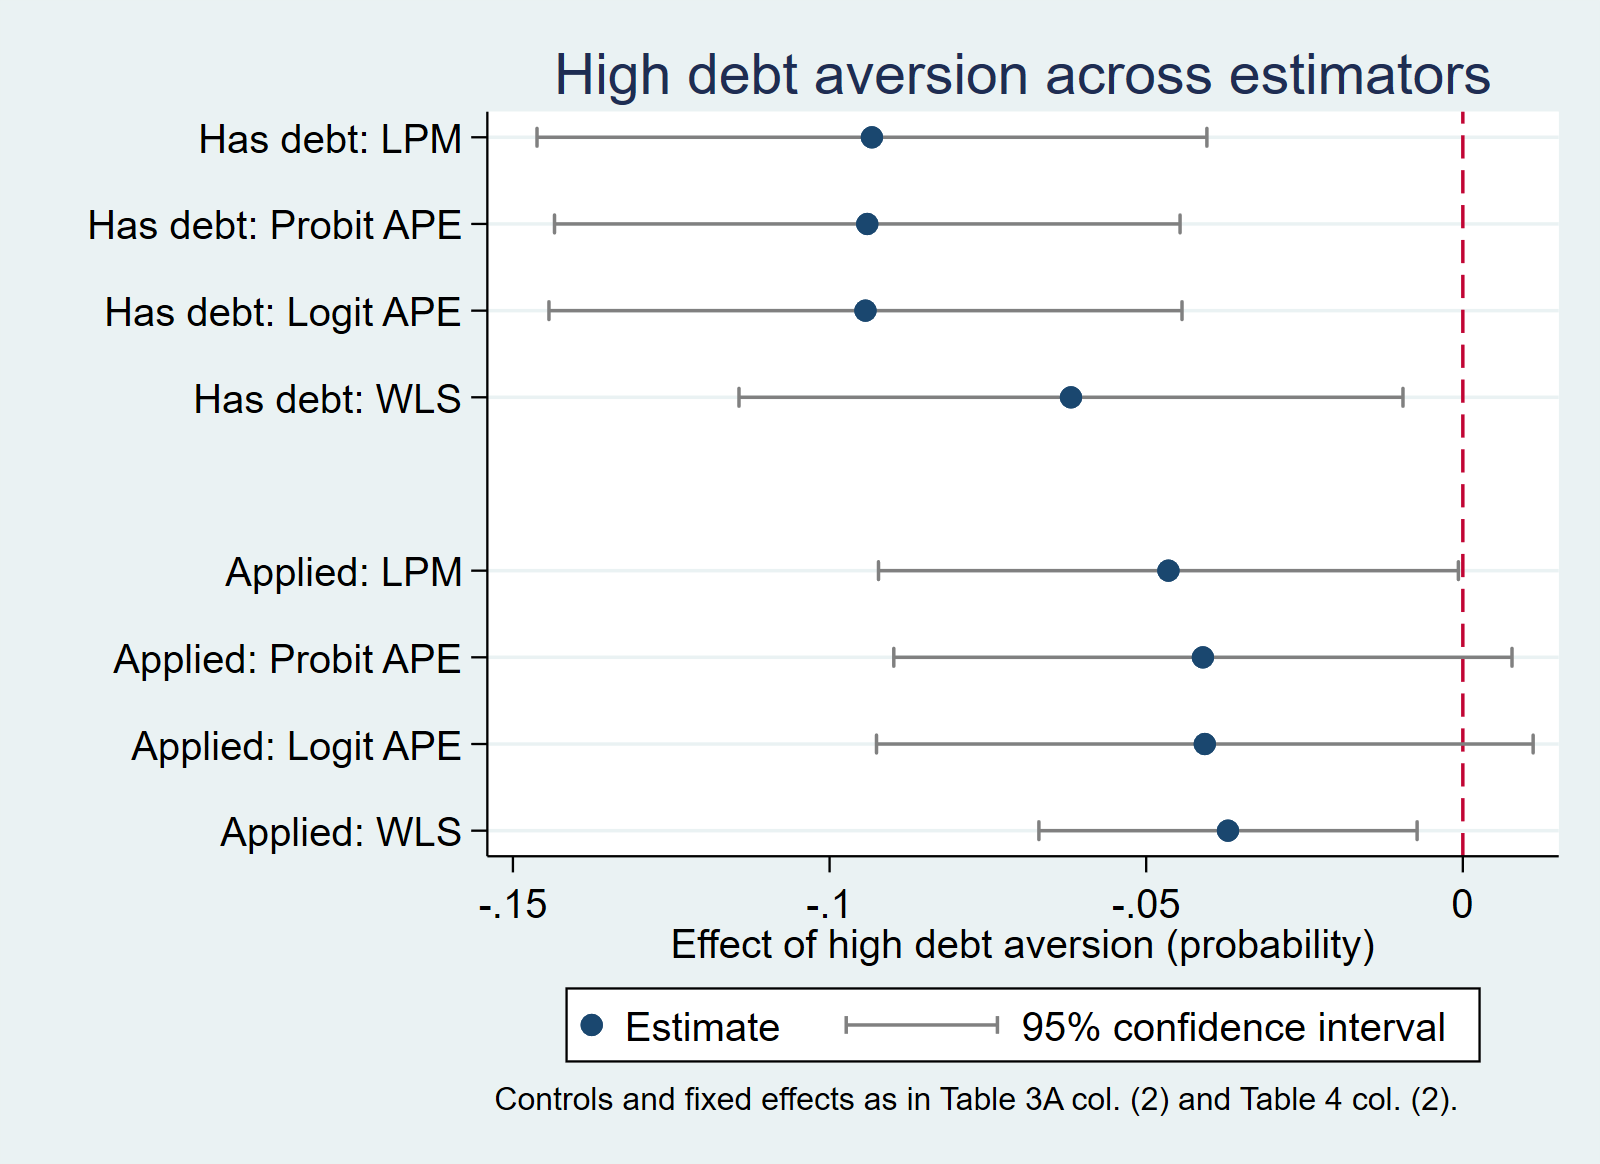
\includegraphics[width=0.75\linewidth]{fig3_estimators.png}
\caption{Effect of High Debt Aversion by Estimator, 2020 Survey}
\label{fig:estimators}
\begin{figurenotes}
Points are the estimates in Table~\ref{tab:estimators}, and the bars are 95 percent confidence intervals from the clustered standard errors. Source: \texttt{output/fig3\_estimates.csv}.
\end{figurenotes}
\end{figure}

H5 is rejected for both outcomes, as the theory predicts. The Breusch-Pagan test gives $F(53, 830) = 1.492$ ($p = 0.015$) for having debt and 2.922 ($p < 0.001$) for the bank loan, and the special White test gives $F = 29.56$ and 72.03 (both $p < 0.001$). Since the standard errors in the paper are already clustered, the inference does not depend on homoskedasticity. However, weighted least squares should be more efficient if the variance is known, and in a linear probability model it is known up to $\hat{y}$. Weighted least squares lowers the debt effect to $-0.062$ (0.027), still significant at 5 percent, and gives $-0.037$ (0.015) for the bank loan, the only model with controls where the loan effect is significant at 5 percent. It is important to note that the weights for the loan model are unreliable, because 142 of the 884 fitted values had to be set to 0.01 before the weights could be computed. Therefore I do not take the weighted loan estimate as stronger evidence than the others.

In the 2023 survey, probit and logit give $-0.196$ and $-0.195$, the same as the linear model. H9 is supported.

\subsection{Functional form: H6}

Is a one point increase in the score worth the same at every point of the scale? Table~\ref{tab:tests} reports the tests. For having debt, the F test of linearity against the score dummies rejects with the usual standard errors ($F(9, 821) = 2.368$, $p = 0.012$), but not with clustered standard errors ($F(9, 43) = 1.668$, $p = 0.127$). The squared score is not significant ($t = -0.794$), and RESET rejects ($F(2, 828) = 4.201$, $p = 0.015$). For the bank loan, linearity is not rejected and the squared score is not significant, but RESET rejects strongly ($F = 15.96$, $p < 0.001$), which points to a problem with the linear probability model itself rather than with the score.

\begin{table}[!htbp]
\centering\small\setlength{\tabcolsep}{5pt}
\caption{Specification Tests}
\label{tab:tests}
\begin{tabular}{llcc}
\toprule
Test & Statistic & Has debt & Applied for bank loan \\
\midrule
Breusch-Pagan & $F(53, 830)$ & 1.492 [0.015] & 2.922 [0.000] \\
Breusch-Pagan & LM, $\chi^2(53)$ & 76.875 [0.018] & 139.020 [0.000] \\
White, special form & $F(2, 881)$ & 29.560 [0.000] & 72.035 [0.000] \\
Linear score vs dummies & $F(9, 821)$ & 2.368 [0.012] & 1.033 [0.412] \\
Linear score vs dummies, clustered & $F(9, 43)$ & 1.668 [0.127] & 1.376 [0.229] \\
Squared score & $t$ (clustered) & $-0.794$ [0.432] & $-0.331$ [0.742] \\
RESET & $F(2, 828)$ & 4.201 [0.015] & 15.960 [0.000] \\
\bottomrule
\end{tabular}
\begin{tablenotes}
$p$-values in brackets. The heteroskedasticity tests use the residuals of column (2) of Table 3A or Table 4. Source: \texttt{output/ext2\_heteroskedasticity.csv}, \texttt{output/ext3\_functional\_form.csv}.
\end{tablenotes}
\end{table}

Figure~\ref{fig:dummies} shows why. Relative to a score of 0, the scores from 1 to 6 have effects close to zero, between $-0.169$ and 0.121 and none significant. The effect turns negative at 7 ($-0.123$, significant at 10 percent), 8 ($-0.129$) and 10 ($-0.165$, both significant at 5 percent), while 9 is close to zero ($-0.015$). In other words, the score works more like a switch that turns on around 7 than a straight line. This supports the paper's choice of a high debt aversion indicator, although its cutoff at 8 leaves out the owners at 7, who behave like the ones above them. H6 is rejected without clustering and not rejected with it, so I read it as weak evidence against linearity.

\begin{figure}[!htbp]
\centering
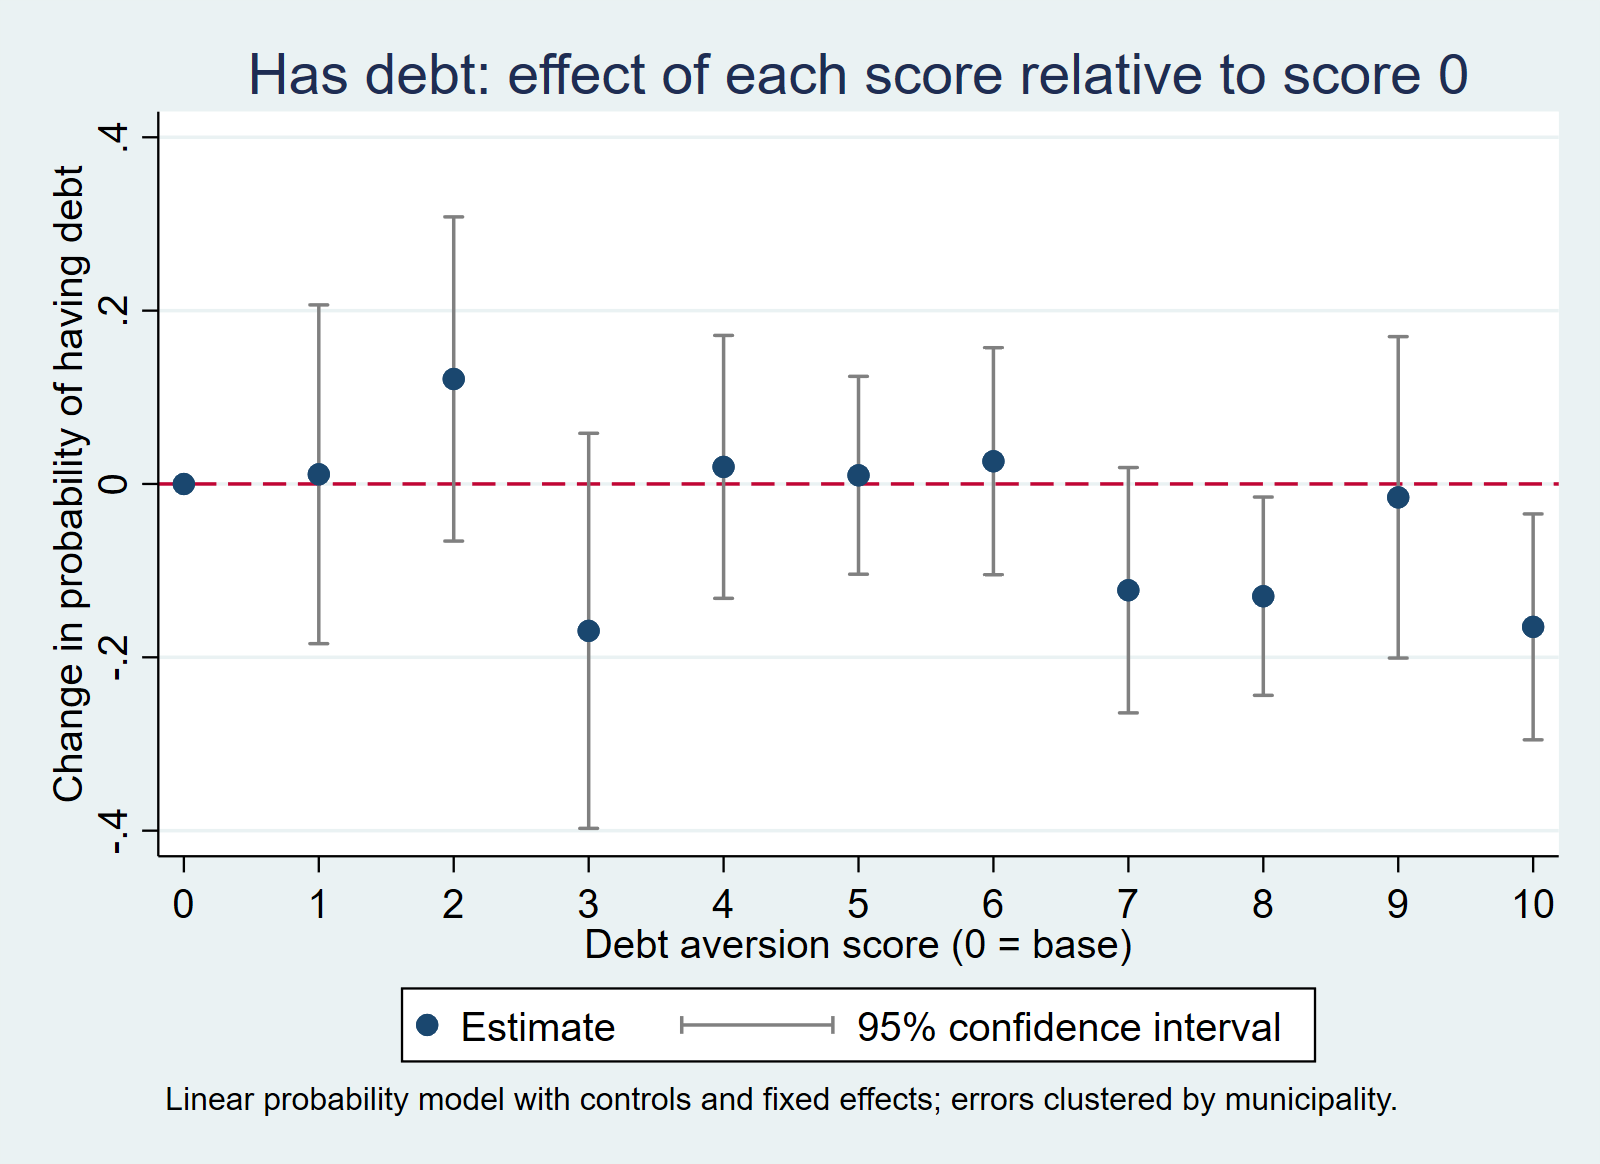
\includegraphics[width=0.62\linewidth]{fig2_score_dummies.png}
\caption{Effect of Each Debt Aversion Score on Having Debt, Relative to a Score of 0}
\label{fig:dummies}
\begin{figurenotes}
Coefficients on the score dummies in the model of column (2) of Table 3A, with 95 percent confidence intervals from clustered standard errors. $N = 884$. Source: \texttt{output/ext3\_score\_dummies\_quadratic.csv}.
\end{figurenotes}
\end{figure}

\subsection{Measurement error: H7}

A single survey question measures an attitude with error, and classical measurement error biases the coefficient on the score toward zero. The survey also asks what the owner was taught about debt as a child, which can serve as instruments for the score. This test is added in the final version of the paper, after instrumental variables are covered in class.

\subsection{Differences across groups: H8}

Table~\ref{tab:groups} reports the interactions. The effect of high debt aversion on having debt does not differ between women and men ($-0.010$, $p = 0.918$) or between firms with 5 or more employees and smaller firms ($-0.015$, $p = 0.779$). The same holds for the bank loan. The Chow test does not reject equal coefficients for women and men. It does reject for firm size ($F(6, 872) = 7.767$ for having debt and 5.055 for the bank loan, both $p < 0.001$), but since the interaction with debt aversion is close to zero, the difference comes from the intercept and the other traits, not from debt aversion. H8 is supported.

\begin{table}[!htbp]
\centering\small\setlength{\tabcolsep}{3pt}
\caption{Effect of High Debt Aversion by Group}
\label{tab:groups}
\begin{tabular}{lcccc}
\toprule
 & \multicolumn{2}{c}{Has debt} & \multicolumn{2}{c}{Applied for bank loan} \\
\cmidrule(lr){2-3}\cmidrule(lr){4-5}
Group variable & Female & Larger firm & Female & Larger firm \\
\midrule
High debt aversion & $-0.089^{*}$ & $-0.088^{**}$ & $-0.026$ & $-0.053^{**}$ \\
 & (0.049) & (0.037) & (0.029) & (0.022) \\
High debt aversion $\times$ group & $-0.010$ & $-0.015$ & $-0.053$ & 0.018 \\
 & (0.094) & (0.052) & (0.033) & (0.041) \\
Female & $-0.006$ & & $-0.004$ & \\
 & (0.086) & & (0.032) & \\
\midrule
Chow test, $F(6, 872)$ & 1.314 [0.248] & 7.767 [0.000] & 0.794 [0.575] & 5.055 [0.000] \\
$N$ & 884 & 884 & 884 & 884 \\
\bottomrule
\end{tabular}
\begin{tablenotes}
Larger firm means 5 or more employees. Its main effect is absorbed by the firm size dummies, so only the interaction is reported. The Chow test compares the intercept, high debt aversion and the four traits across the two groups, with the dummies kept common. Clustered standard errors in parentheses, $p$-values in brackets. $^{*}p<0.10$, $^{**}p<0.05$, $^{***}p<0.01$. Source: \texttt{output/ext5\_group\_interactions.csv}, \texttt{output/ext5\_group\_tests.csv}.
\end{tablenotes}
\end{table}

\section{Limitations and Conclusion}

\subsection{Limitations}

The data are one survey at one point in time, and debt aversion, the outcomes and the traits are all reported by the owner. An owner who has avoided debt for years may say afterward that debt is unpleasant, so the direction of the effect cannot be settled with this design, and the paper's survey experiment, which I do not replicate, is its main answer to that concern. The sample is Finnish and from a single crisis, where support came through banks, so the effect may be different where support came as grants. The paper's Table 3B cannot be replicated because the Orbis ratios were removed from the package. With 44 clusters the clustered standard errors are reliable but not exact, and the RESET test shows the linear probability model is not a perfect fit for the bank loan. Finally, one author's funding came in part from a foundation linked to a Finnish bank group, which I note for completeness; it does not change any number here.

\subsection{Conclusion}

I replicate the main results of Paaso, Pursiainen and Torstila (2025) with the authors' survey data and my own Stata code. Owners with high debt aversion are 9.3 percentage points less likely to have debt, against 9.4 in the paper, and all 18 coefficients I compare match the paper to within 0.001. The extension shows the debt use result is strong. It is the same in probit and logit, it survives weighted least squares at a smaller size, it is not driven by group differences, and it is twice as large in the 2023 survey. The score behaves like a threshold at 7 and above, which supports the paper's use of an indicator.

However, the result on bank loan applications during COVID-19, which is the one most relevant for policy, is weaker. It is significant only at the 10 percent level in the paper's model, it is not significant in the logit, and the linear model predicts negative probabilities for 142 firms. A next step would be to estimate the loan decision only for firms that faced a large sales shock, where the need for credit is clearest, and to use the 2023 survey's question on loans and grants.

The coefficients in a paper tell us what the data say only after the assumptions behind them have been tested, and here the tests are what separated the strong result from the weak one.

\begin{thebibliography}{00}

\bibitem[Paaso et al.(2025)]{paaso2025} Paaso, Mikael, Vesa Pursiainen, and Sami Torstila. 2025. Entrepreneur debt aversion and financing decisions: Evidence from COVID-19 support programs. \textit{Management Science} 72 (5), 4474-4498. Replication data at \url{https://doi.org/10.1287/mnsc.2022.03007}.

\bibitem[Wooldridge(2020)]{wooldridge} Wooldridge, Jeffrey M. 2020. \textit{Introductory Econometrics: A Modern Approach}. 7th ed. Boston: Cengage.

\end{thebibliography}

\vspace{6pt}
\noindent Code: \href{https://github.com/nowshed-imran/ECON-5213-Project}{github.com/nowshed-imran/ECON-5213-Project}

\end{document}
